\chapter{Introducción específica} % Main chapter title

\label{Chapter2}

%----------------------------------------------------------------------------------------
%	SECTION 1
%----------------------------------------------------------------------------------------
En este capítulo se introduce la terminología de la red de comunicaciones del tren y del sistema de información al pasajero. Se incluye una descripción de su arquitectura y de sus módulos principales. Se presenta también el detalle del sistema que maneja los carteles led que presentan información al pasajero en los coches de las formaciones ferroviarias de Trenes Argentinos.\\



\section{Trenes: Redes de comunicación TCN}

La red de comunicaciones del tren (TCN) presenta una arquitectura de buses jerárquicos de dos niveles que se pueden identificar en la figura 1: el bus de datos WTB y el MVB [IEC-61375,1999]. El WTB se encarga de las comunicaciones entre coches a través de nodos con redundancia física, mientras que al bus MVB se conectan los dispositivos de cada coche. Algunos de estos dispositivos son el control de puertas (DOORL/R), el aire acondicionado (HVAC), el sistema de tracción (VVVF), el sistema de control de frenos (BCU), entre otros. El mapa de recorrido y los carteles LED en conjunto con otros dispositivos como los parlantes y las cámaras de video (CCTV) forman un sistema denominado Sistema de información al pasajero (PIDS).



\begin{figure}[ht]
	\centering
	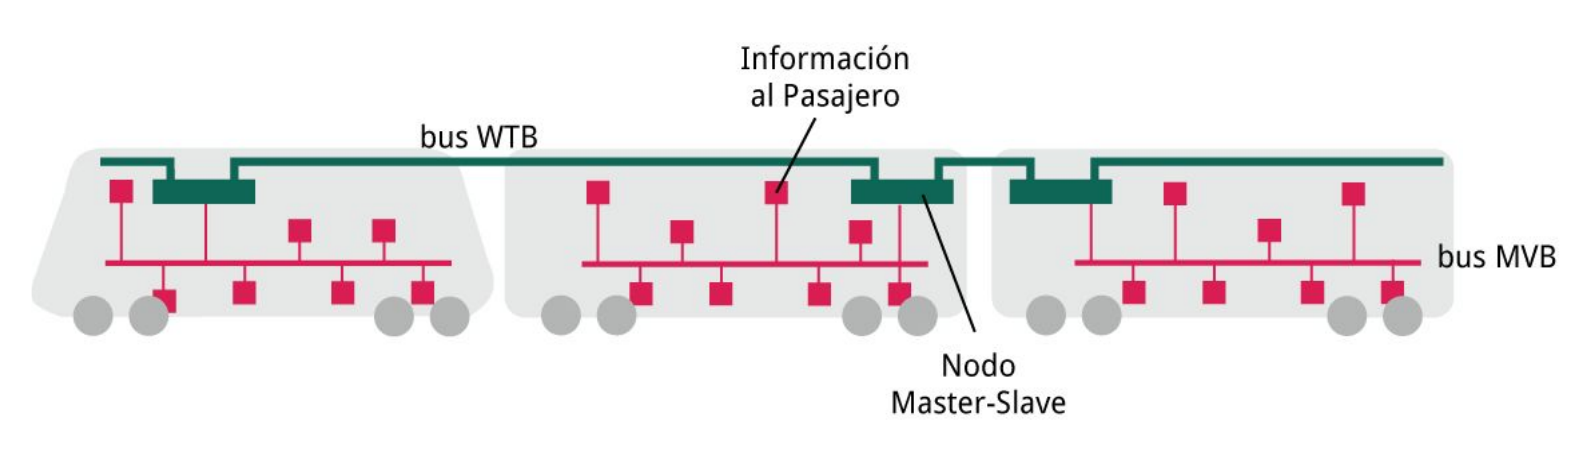
\includegraphics[width=1\textwidth]{./Figures/diagramaRedTCN.png}
	\caption{}
	\label{fig:redTCN}
\end{figure}


\begin{figure}[ht]
	\centering
	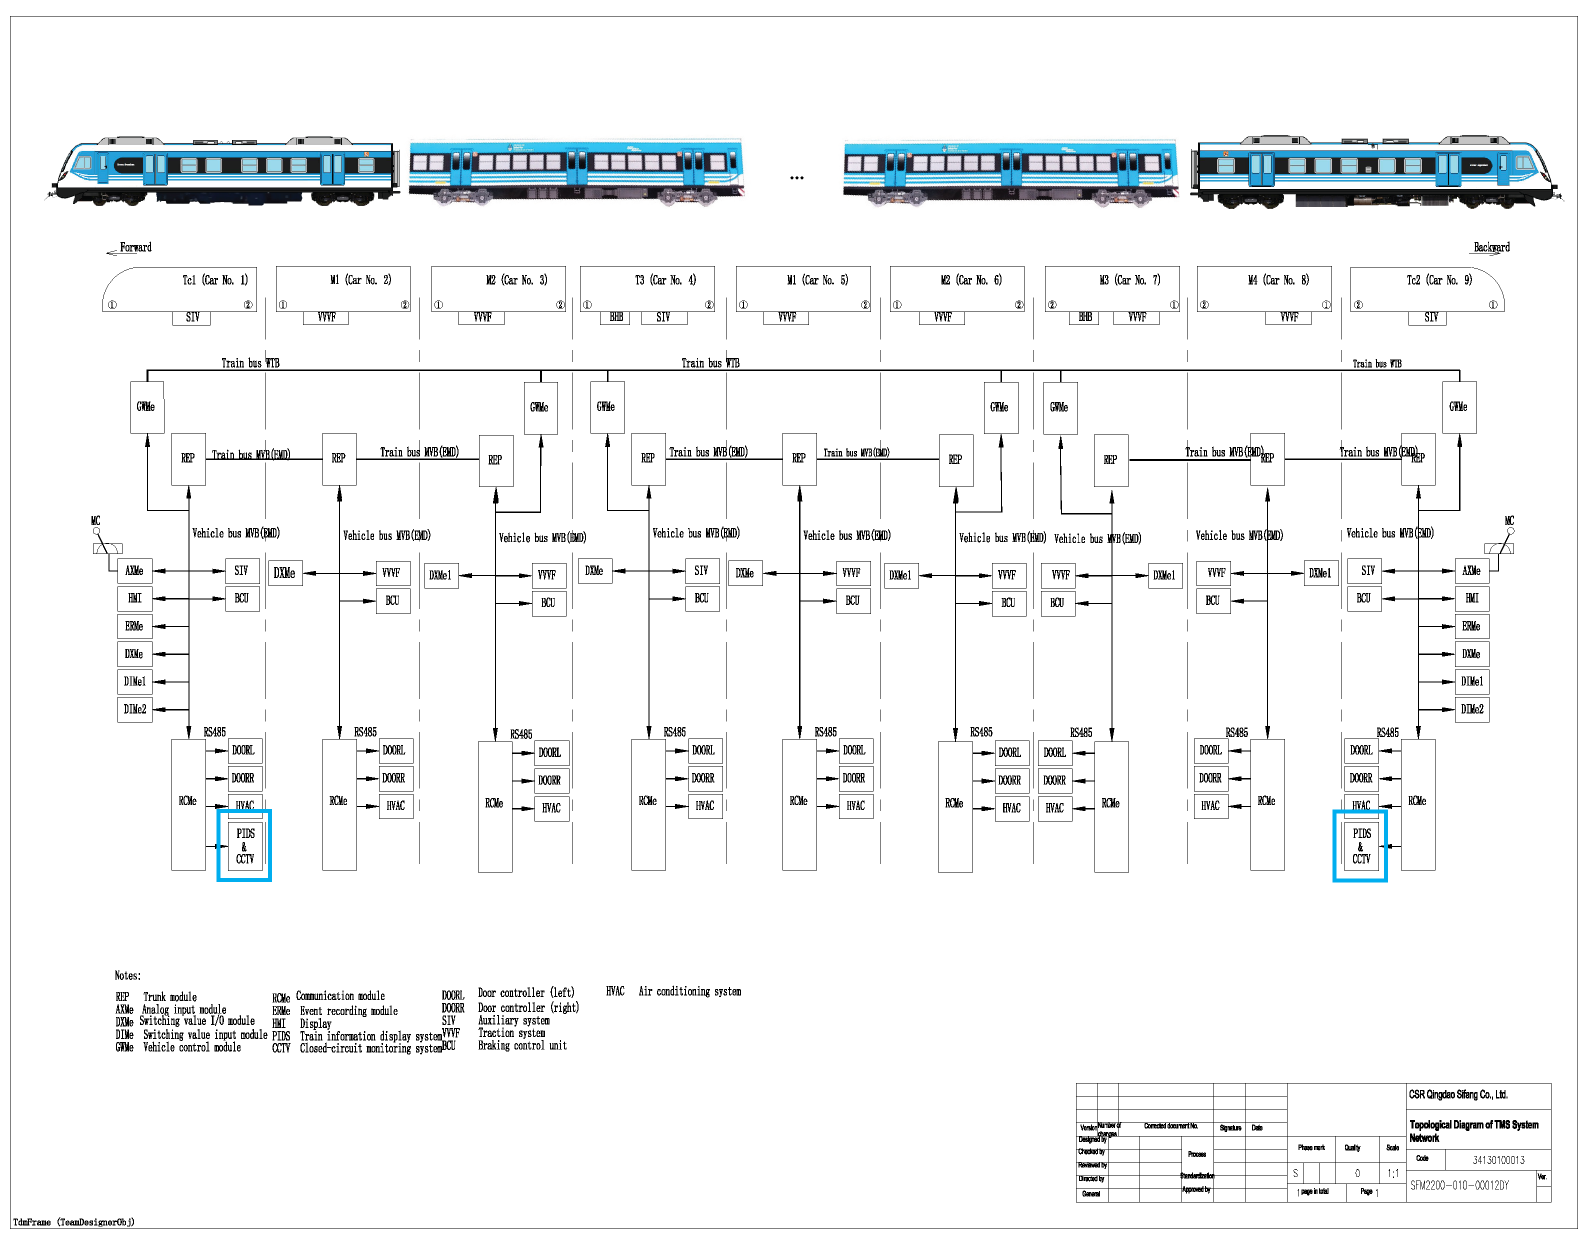
\includegraphics[width=1\textwidth]{./Figures/diagramaTrenesArgentinosTCN.png}
	\caption{}
	\label{fig:sofseTCN}
\end{figure}


\begin{figure}[ht]
	\centering
	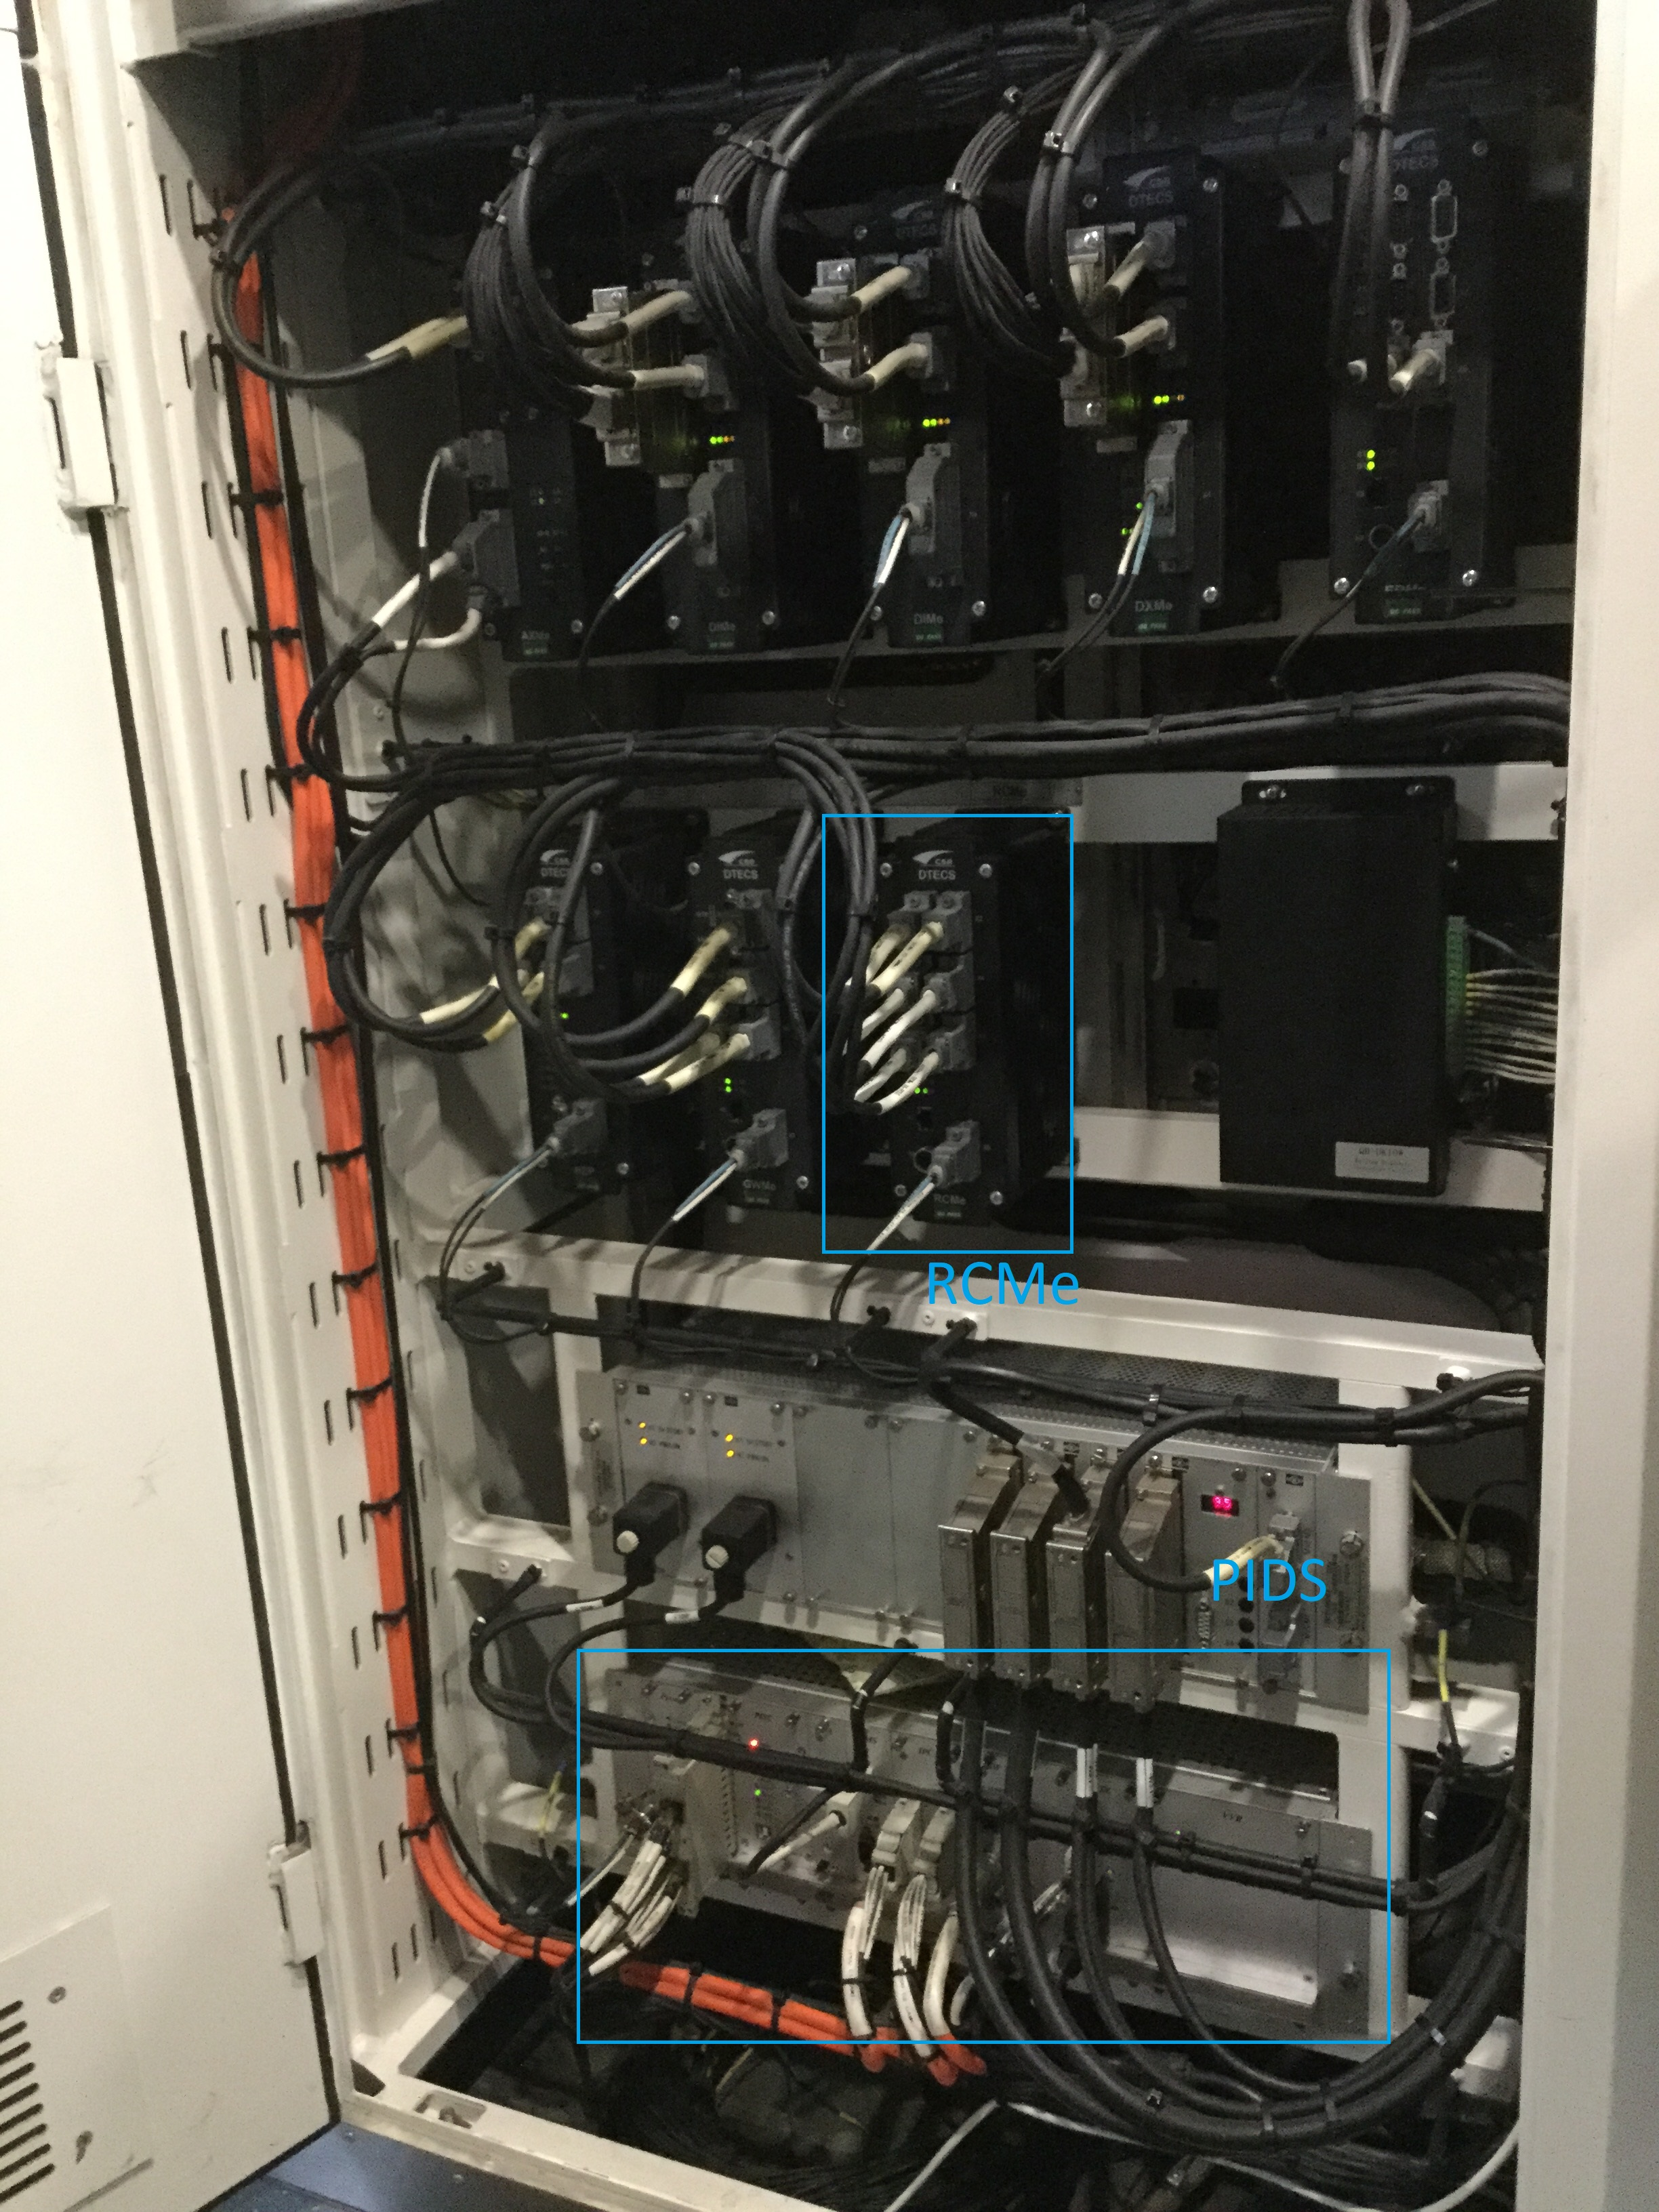
\includegraphics[width=1\textwidth , angle=90]{./Figures/imgRackTCN.JPG}
	\caption{}
	\label{fig:imgRackTCN}
\end{figure}



\pagebreak
\section{PIDS: Sistema de información visual para pasajeros de trenes}

\begin{figure}[ht]
	\centering
	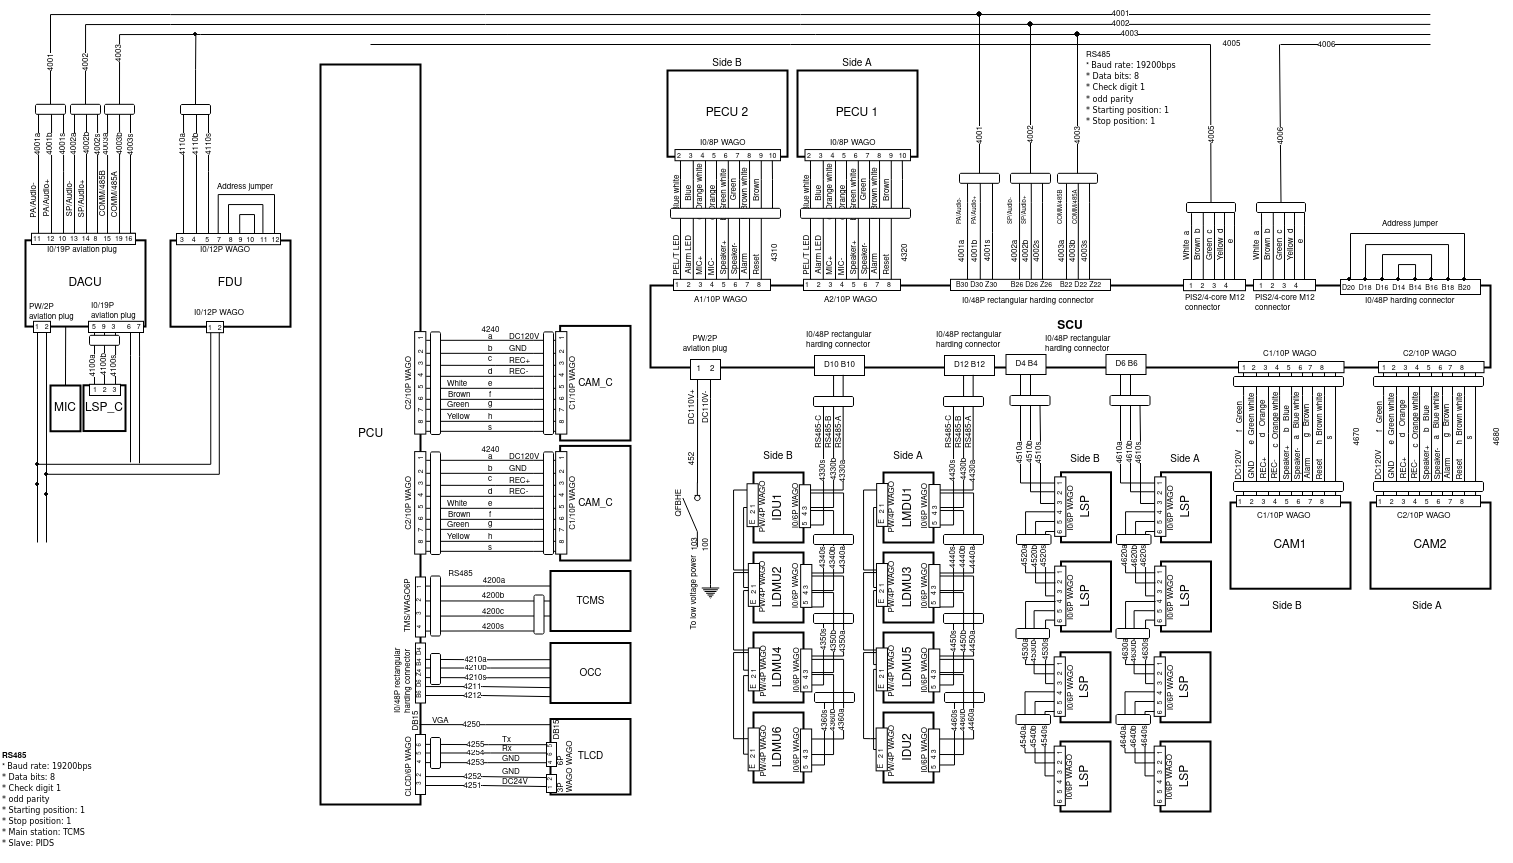
\includegraphics[width=1\textwidth , angle=90]{./Figures/diagramaPIDS.png}
	\caption{}
	\label{fig:diagramaPIDS}
\end{figure}


\begin{figure}[ht]
	\centering
	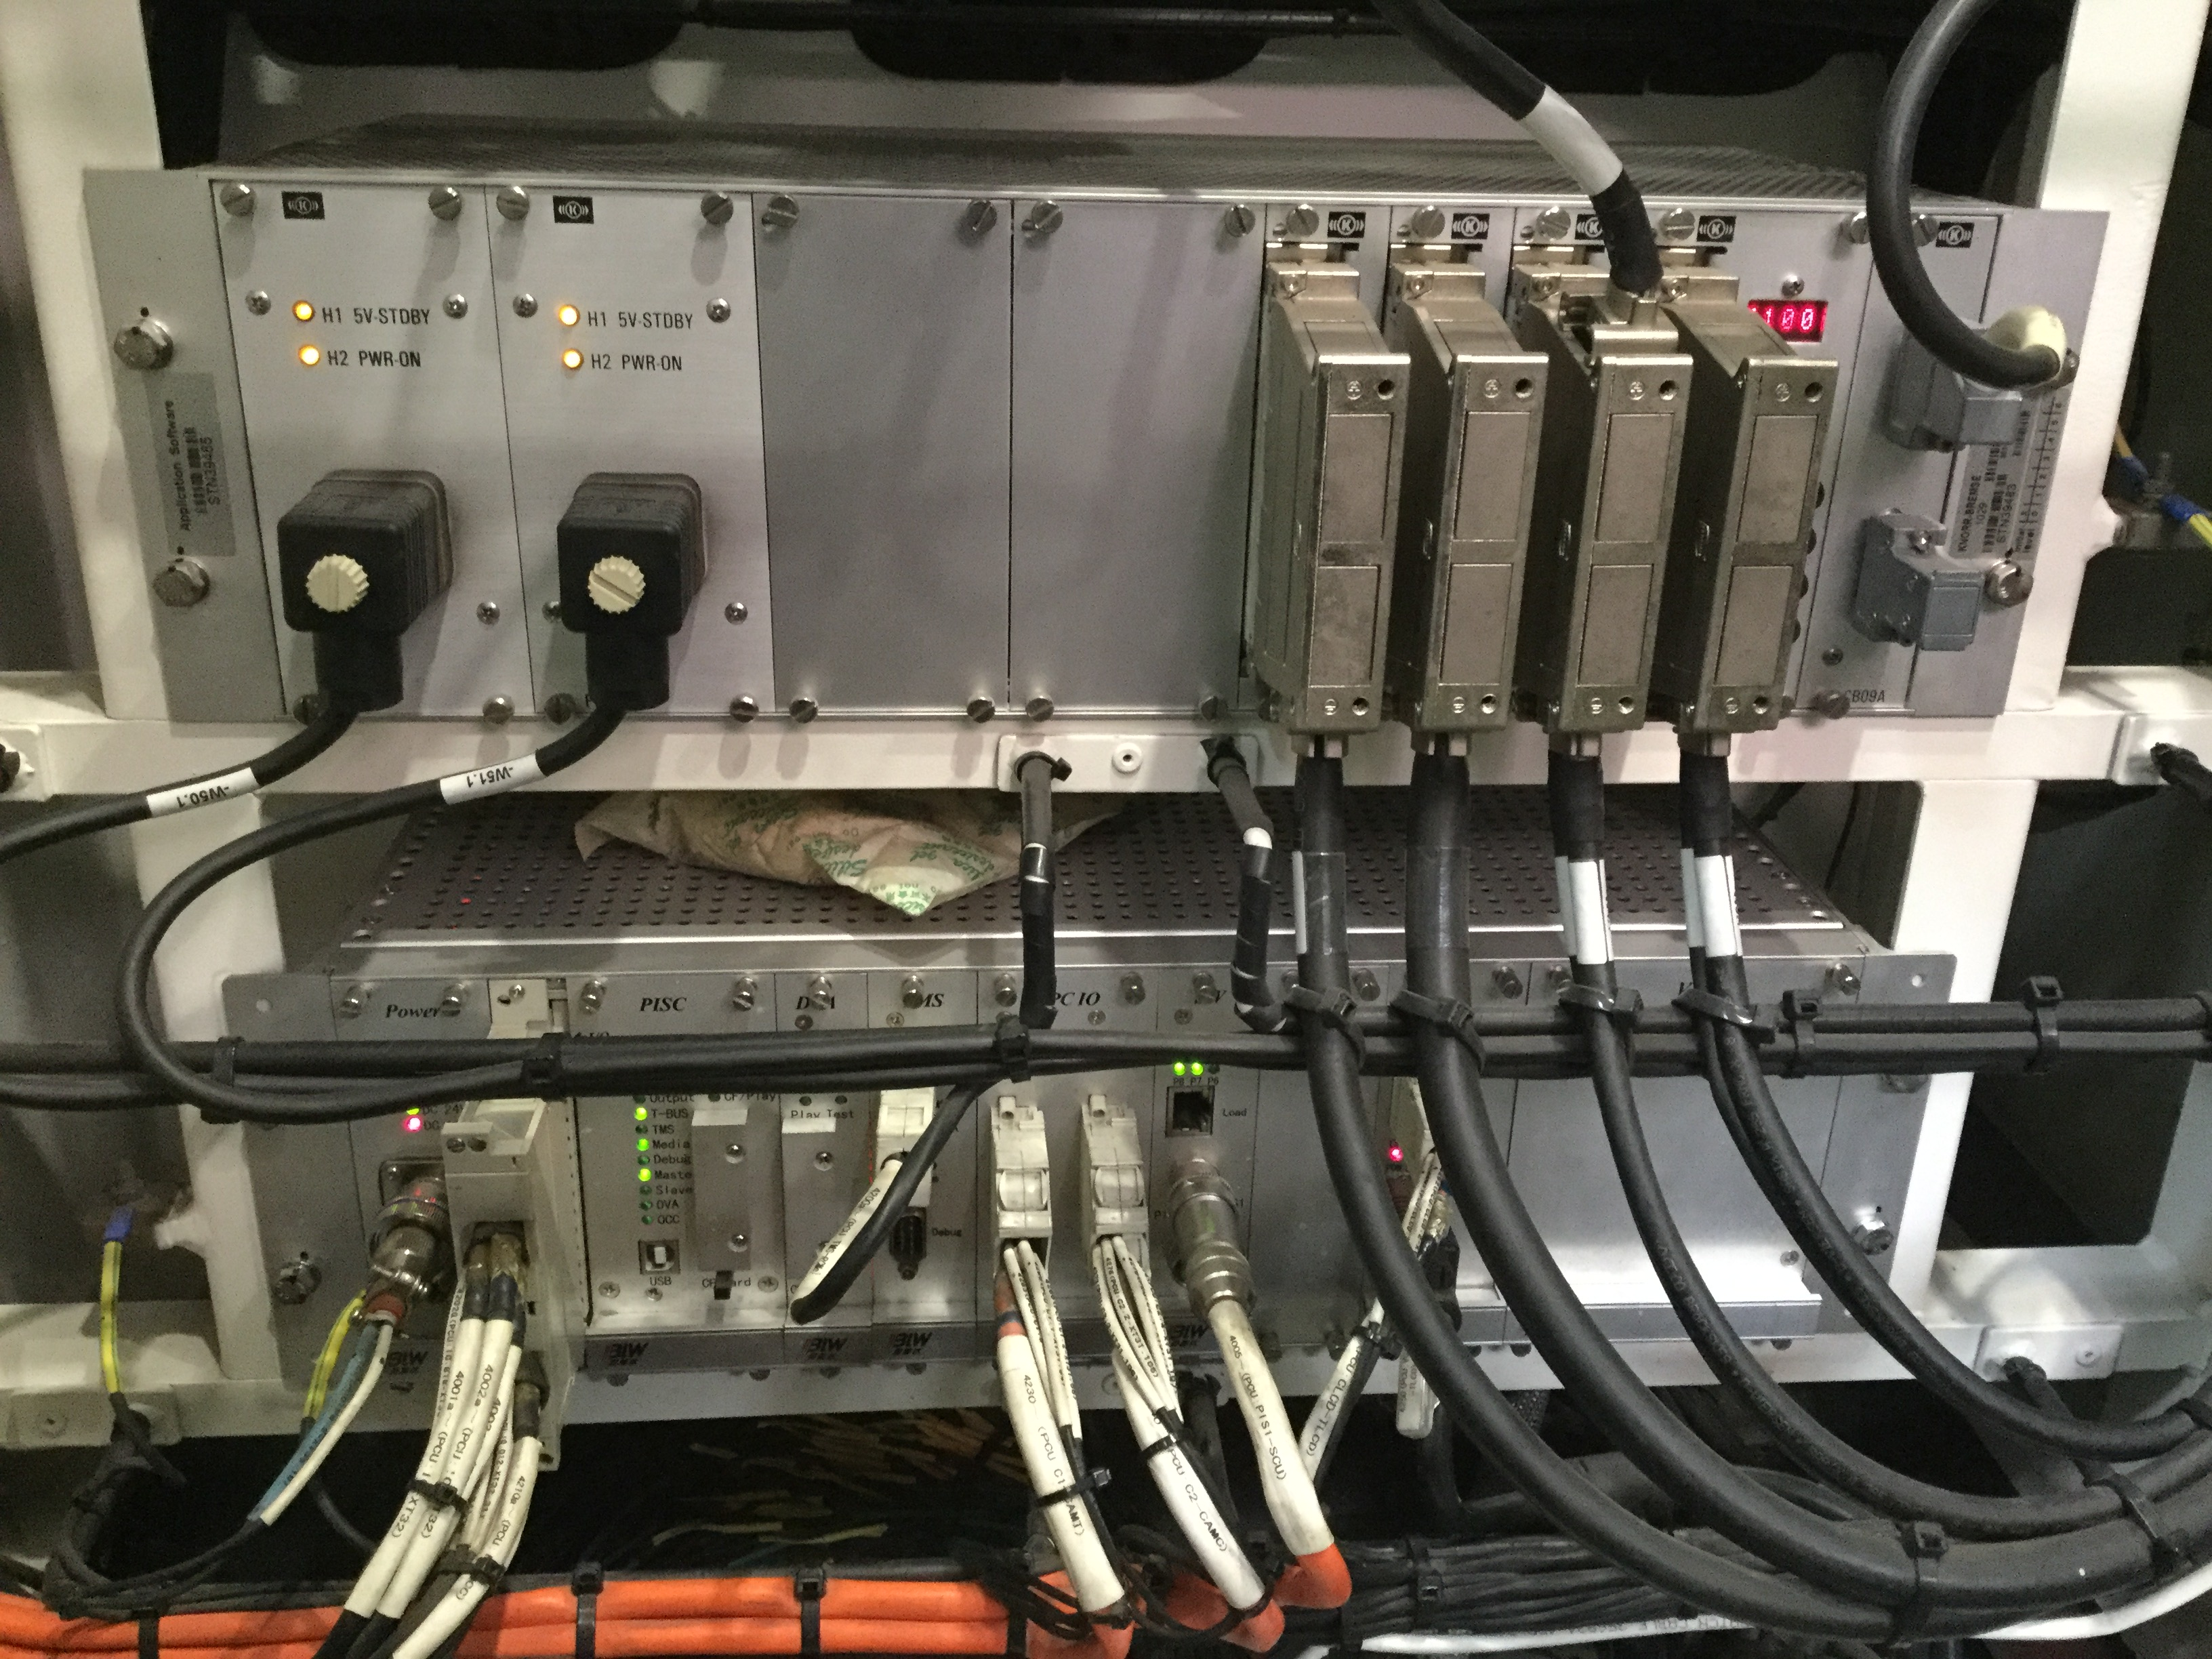
\includegraphics[width=1\textwidth , angle=90]{./Figures/rackPIDS1.JPG}
	\caption{}
	\label{fig:rackPIDS1}
\end{figure}


\begin{figure}[ht]
	\centering
	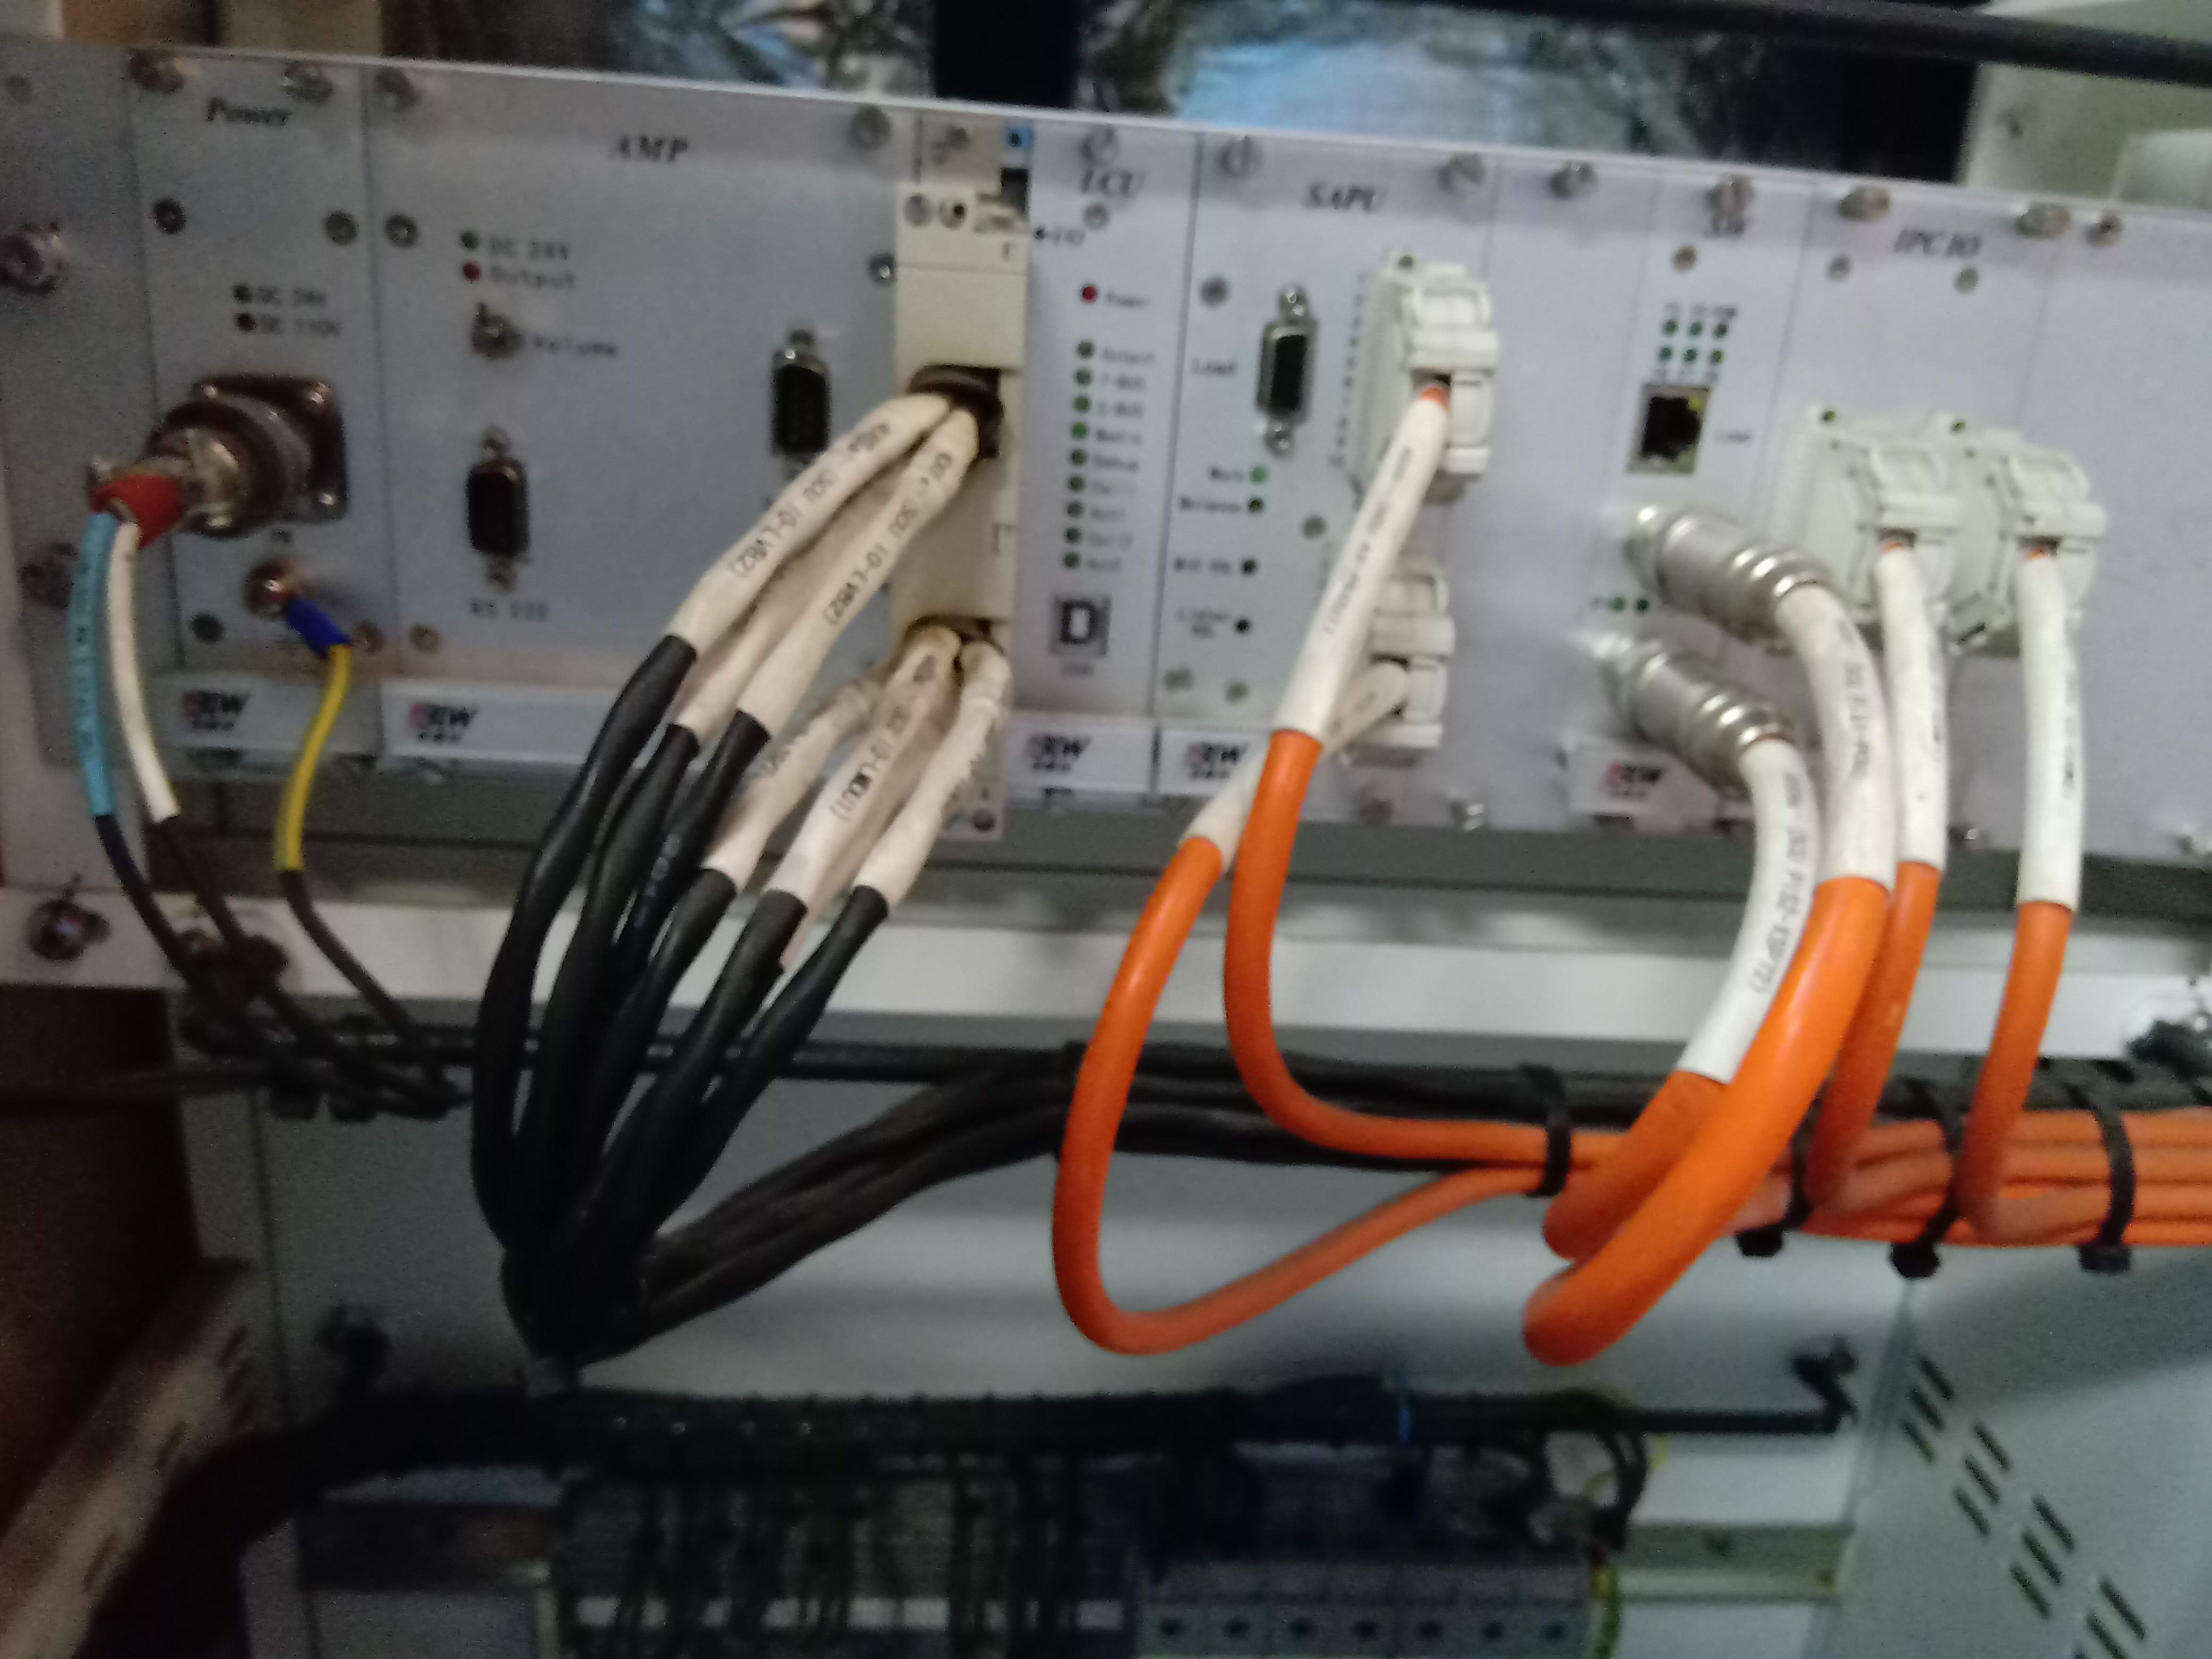
\includegraphics[width=1\textwidth , angle=90]{./Figures/rackPIDS2.jpg}
	\caption{}
	\label{fig:rackPIDS2}
\end{figure}


\pagebreak
\section{Carteles y controladoras de matrices LED}

\begin{figure}[ht]
	\centering
	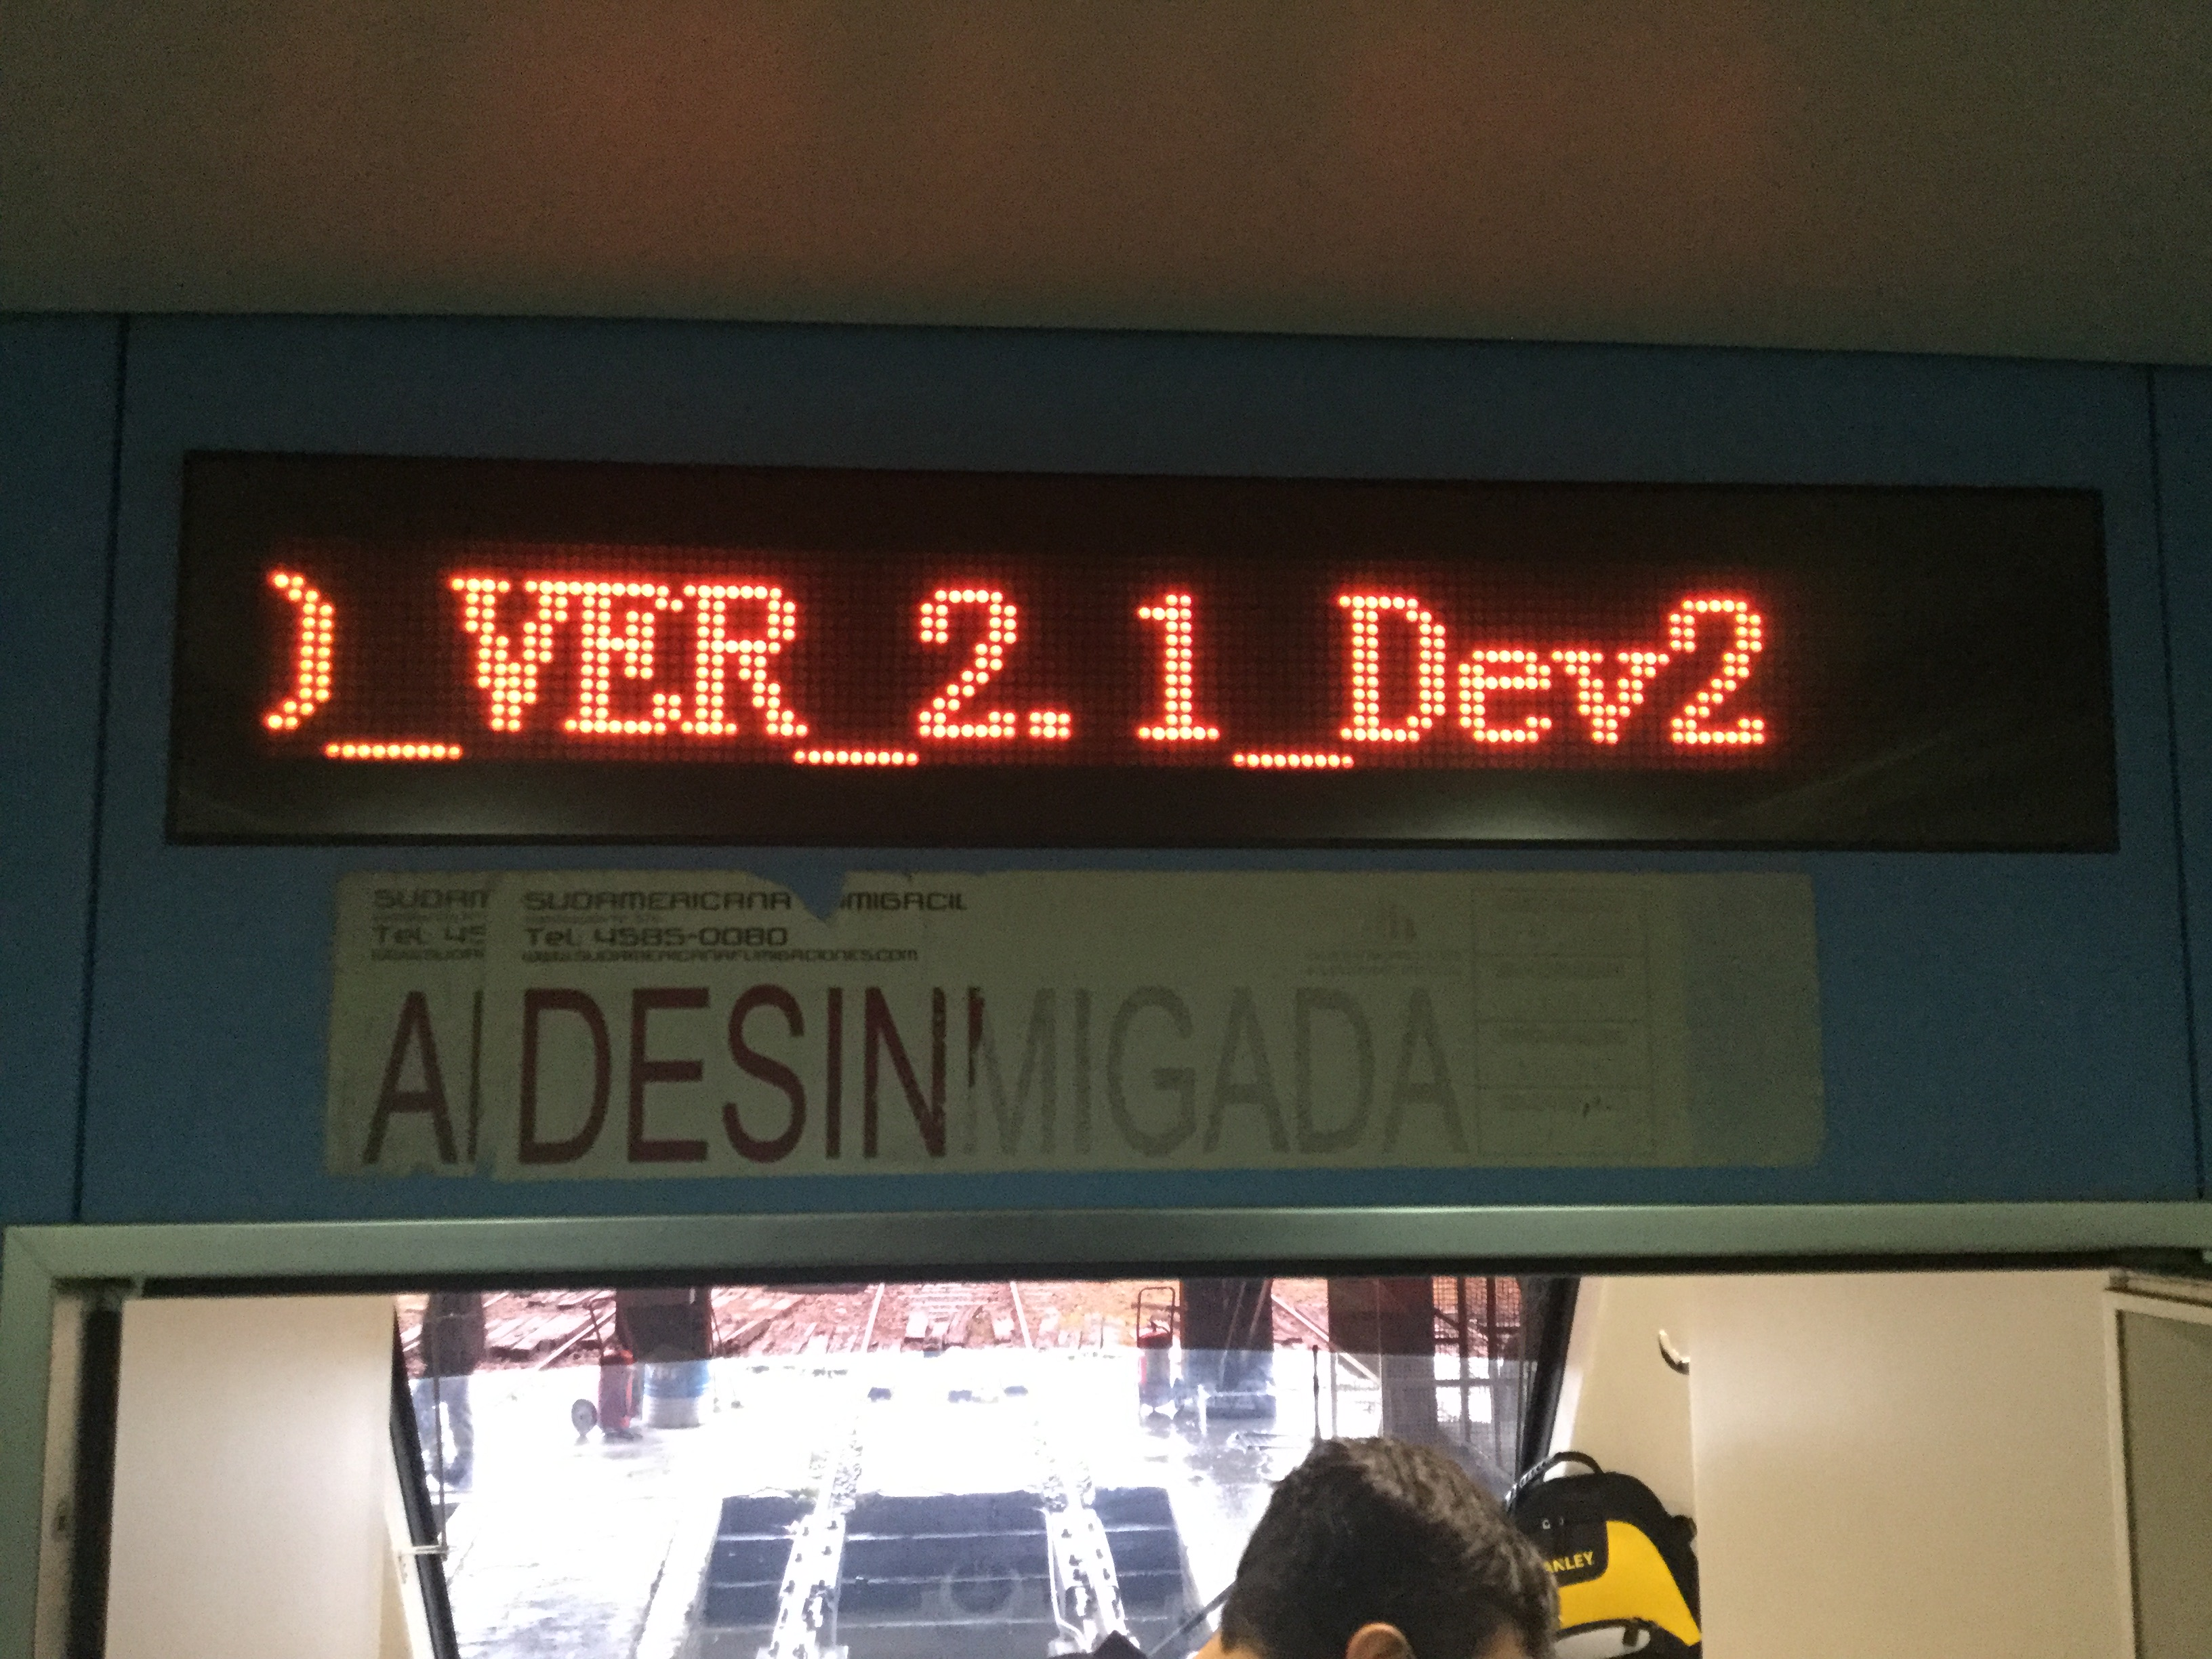
\includegraphics[width=1\textwidth]{./Figures/cartelIniciando.JPG}
	\caption{}
	\label{fig:cartelIniciando}
\end{figure}

\begin{figure}[ht]
	\centering
	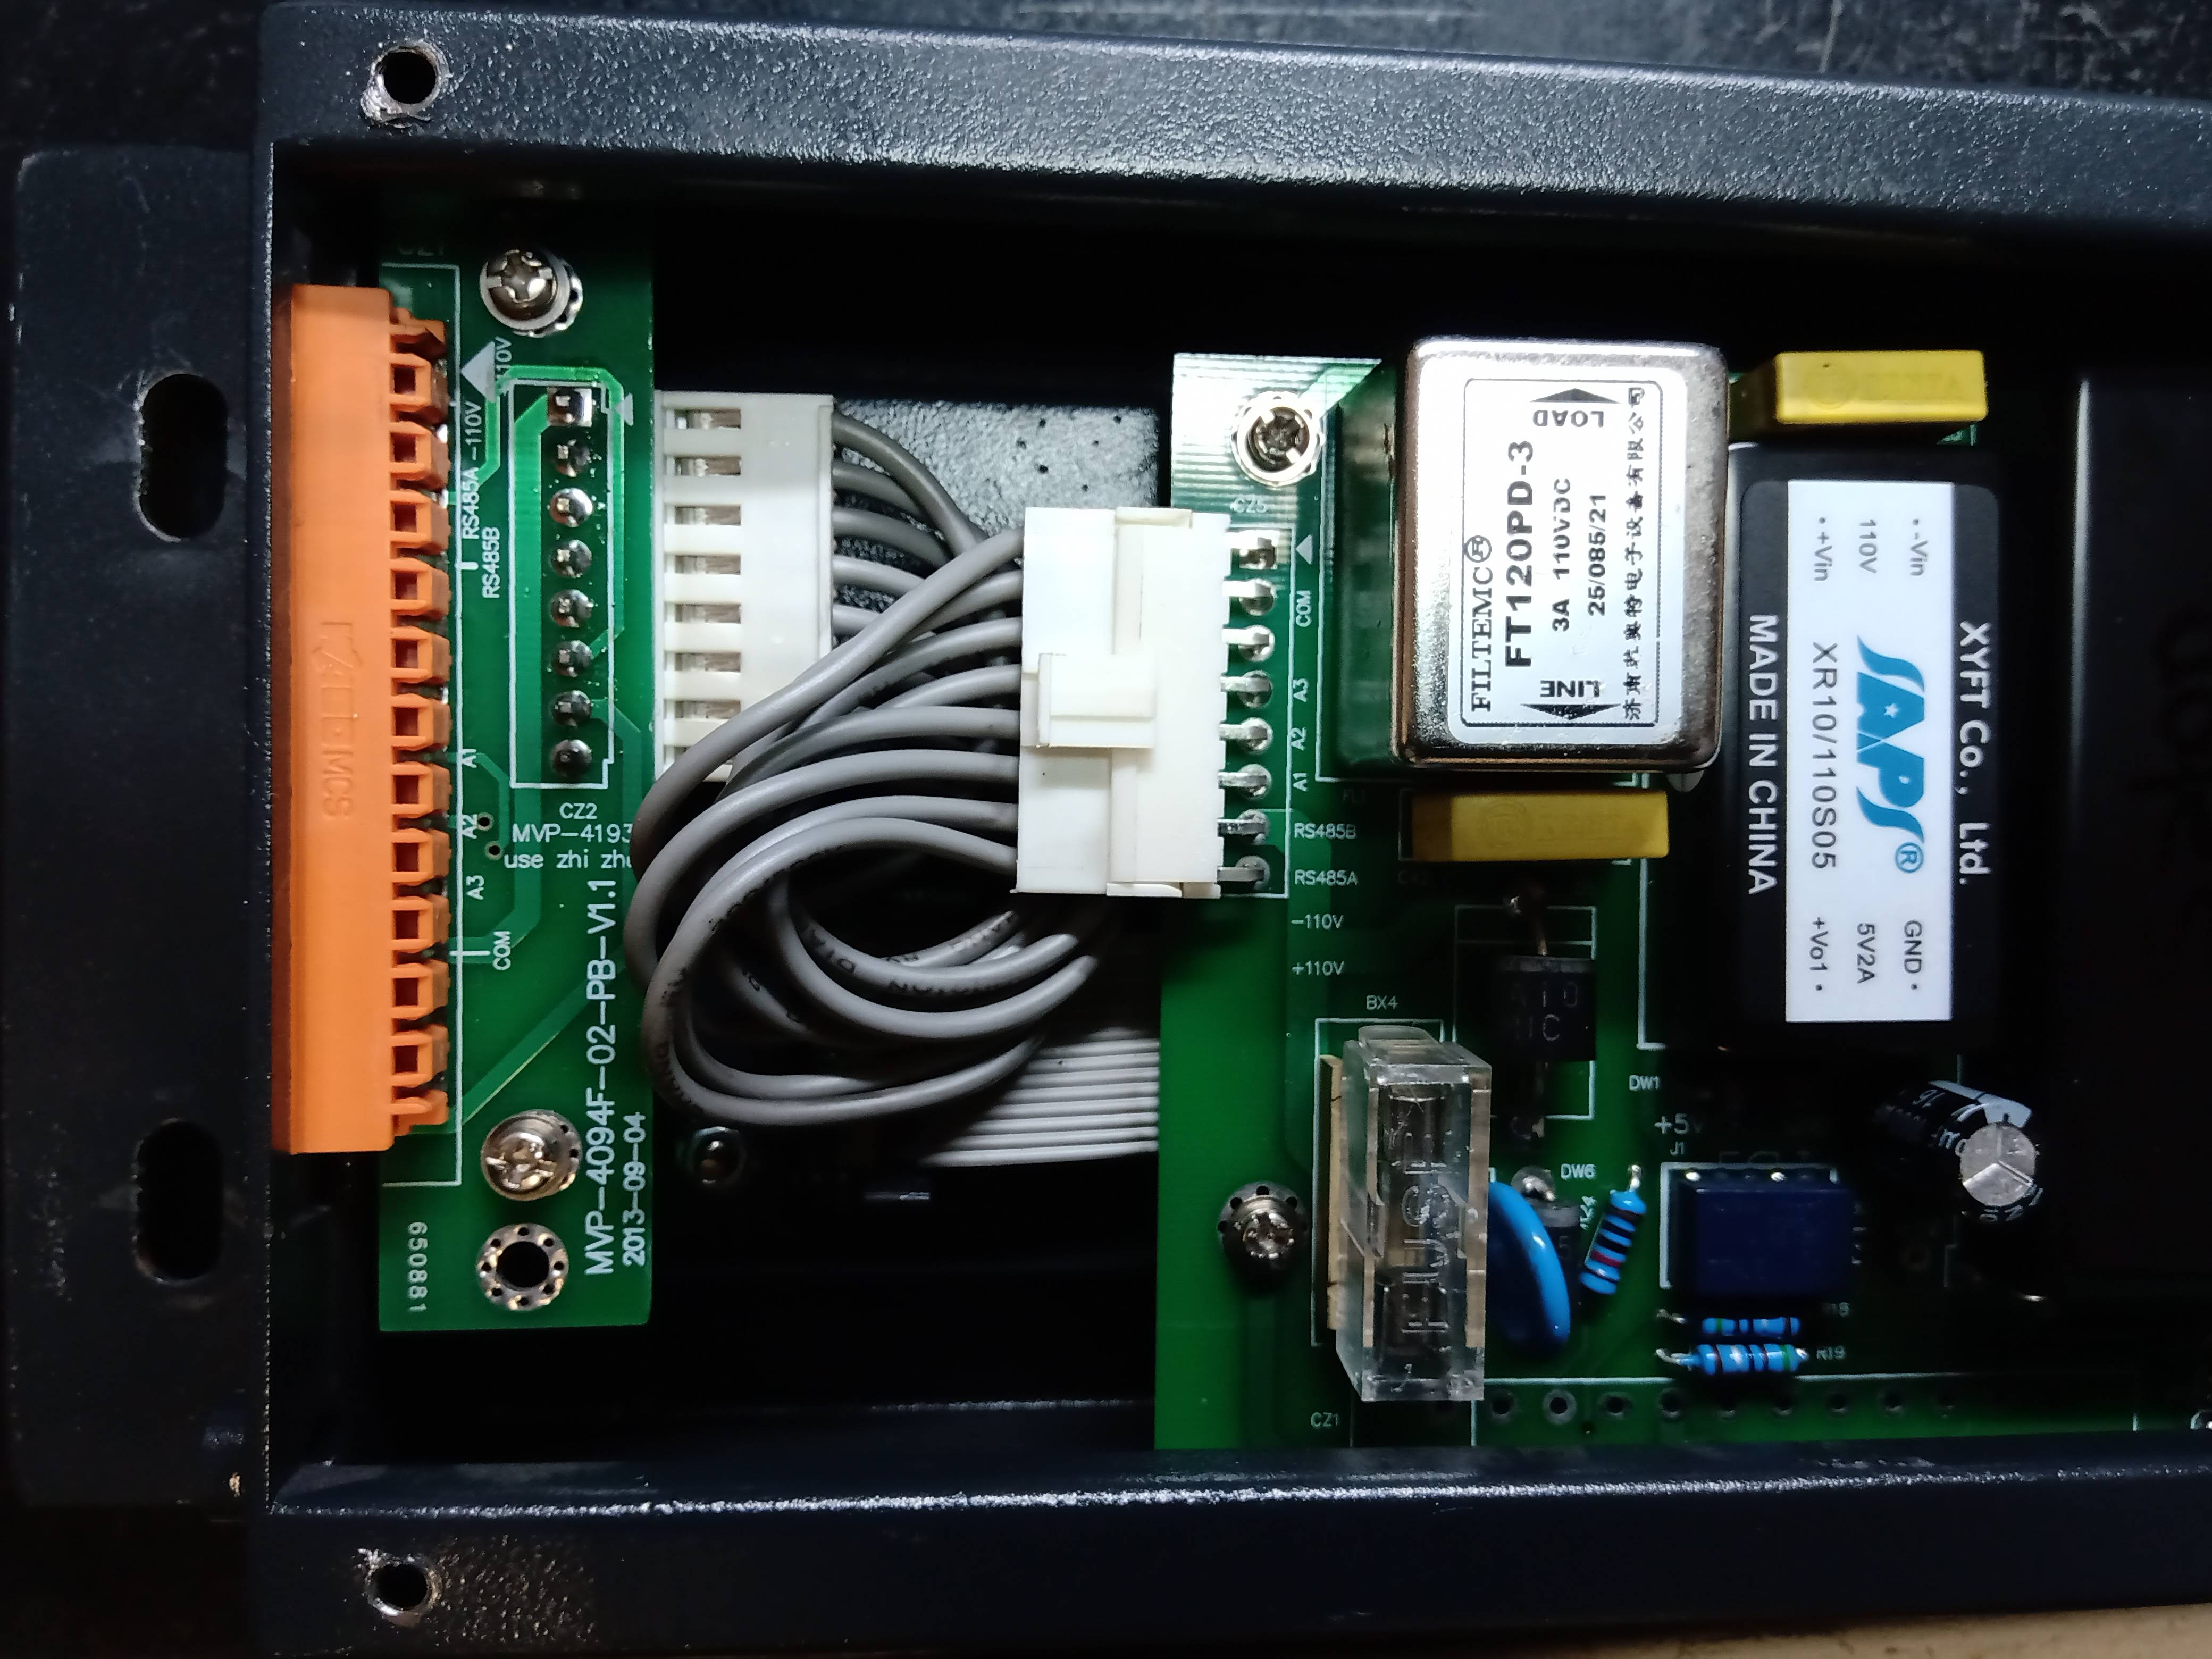
\includegraphics[width=1\textwidth]{./Figures/displayController.jpg}
	\caption{}
	\label{fig:displayController}
\end{figure}
